\section[Potenzen und Logarithmen]{Potenzen und Logarithmen \bronstein{8}}
%Rechenregeln
\begin{minipage}[t]{0.5\textwidth}
	\subsection{Potenzen}
	\begin{tabular}{ll}
		$a^{0}=1$ & $a^{-n}=\frac{1}{a^{n}}$\\
		$a^{\frac{m}{n}}=\sqrt[n]{a^{m}}$ & $\left(a^{r}\right)^{s}=a^{r \cdot s}$\\
		$a^{r+s}=a^{r} \cdot a^{s}$ & $a^{r-s}=\frac{a^{r}}{a^{s}}$\\
		$(a \cdot b)^{r}=a^{r} \cdot b^{r}$ & $\left(\frac{a}{b}\right)^{r}=\frac{a^{r}}{b^{r}}$\\
	\end{tabular}
%
	\subsection{Logarithmen}
	\begin{tabular}{ll}
		$a^x = b \rightarrow x = \log_{a}(b)$				&\\
															&\\
		$\log _{b}(x \cdot y)=\log _{b} (x)+\log _{b} (y)$ 	& $\log _{b} (\frac{x}{y})=\log _{b} (x)-\log _{b} (y)$\\
		$\log _{b} (\frac{1}{x})=-\log _{b} (x)$ 			& $\log _{b} (\frac{x}{y})=-\log _{b} (\frac{y}{x})$\\
		$\log _{b}\left(x^{r}\right)=r \log _{b} (x)$ 		& $\log _{b} (\sqrt[n]{x})=\frac{1}{n} \log _{b} (x)$\\
		$\log _{b} (x)=\frac{\log _{a} (x)}{\log _{a} (b)}$ & $\log _{e} (x)=\ln(x)$
	\end{tabular}
\end{minipage}
%
% Grafik
\begin{minipage}[t]{0.5\textwidth}
	\begin{flushright}
		\strut\vspace*{-\baselineskip}\newline
		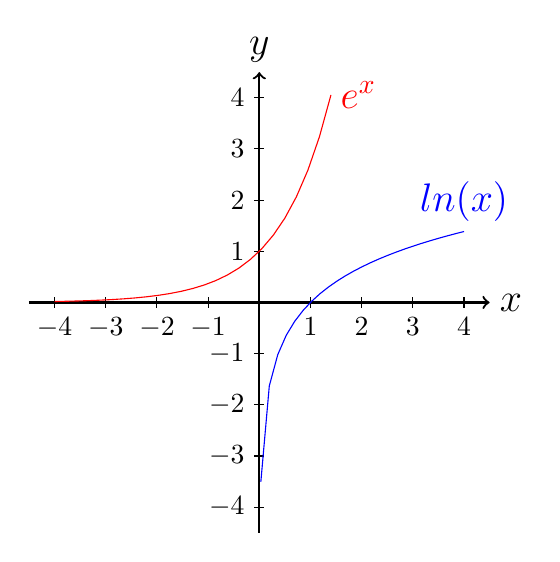
\begin{tikzpicture}[xscale=0.65, yscale=0.65]
	%axis
	\draw[thick, ->] (-4.5, 0) -- (4.5,0) node[right] {\Large $x$};
	\draw[thick, ->] (0, -4.5) -- (0,4.5) node[above] {\Large $y$};
	%
	%grid x
	\draw (-4, -0.1) node[below]{$-4$} -- (-4, 0.1);
	\draw (-3, -0.1) node[below]{$-3$} -- (-3, 0.1);
	\draw (-2, -0.1) node[below]{$-2$} -- (-2, 0.1);
	\draw (-1, -0.1) node[below]{$-1$} -- (-1, 0.1);
	\draw (1, -0.1) node[below]{$1$} -- (1, 0.1);
	\draw (2, -0.1) node[below]{$2$} -- (2, 0.1);
	\draw (3, -0.1) node[below]{$3$} -- (3, 0.1);
	\draw (4, -0.1) node[below]{$4$} -- (4, 0.1);
	%grid y
	\draw (-0.1, 4) node[left]{$4$} -- (0.1, 4);
	\draw (-0.1, 3) node[left]{$3$} -- (0.1, 3);
	\draw (-0.1, 2) node[left]{$2$} -- (0.1, 2);
	\draw (-0.1, 1) node[left]{$1$} -- (0.1, 1);
	\draw (-0.1, -1) node[left]{$-1$} -- (0.1, -1);
	\draw (-0.1, -2) node[left]{$-2$} -- (0.1, -2);
	\draw (-0.1, -3) node[left]{$-3$} -- (0.1, -3);
	\draw (-0.1, -4) node[left]{$-4$} -- (0.1, -4);
	%
	%plots
	\draw[red, domain=-4:1.4] plot (\x, {e^\x}) node[right, red] {\Large $e^x$};
	\draw[blue, domain=0.03:4] plot (\x, {ln(\x)})node[above, blue] {\Large $ln(x)$};
\end{tikzpicture}
	\end{flushright}
\end{minipage}

\subsection{dB-Rechnung}
%\textbf{Linear nach Dezibel (dB):}\\
\begin{minipage}[t]{0.48\textwidth}
	\renewcommand{\arraystretch}{1.5}
	\begin{tabular}{|ll|}
		\hline
		\multicolumn{2}{|c|}{\textbf{Linear nach Dezibel(dB):}}\\
		\textbf{Leistung} & \textbf{Amplituden}\\
		$P_{dB} = 10 \cdot log\left(\dfrac{P_2}{P_1}\right)$ & $A_{dB} = 20 \cdot log\left(\dfrac{A_2}{A_1}\right)$\\
		\multicolumn{2}{|c|}{\textbf{Dezibel(dB) nach Linear:}}\\
		\textbf{Leistung} & \textbf{Amplituden}\\
		$\dfrac{P_2}{P_1} = 10^{\frac{P_{dB}}{10}}$ & $\dfrac{A_2}{A_1} = 10^{\frac{A_{dB}}{20}}$\\
		\quad & \quad\\
		\hline
	\end{tabular}
	\renewcommand{\arraystretch}{1}
\end{minipage}
%
\hspace{0.04\textwidth}
%
\begin{minipage}[t]{0.48\textwidth}
	\renewcommand{\arraystretch}{1.3}
	\begin{tabular}{|c|c|c|}
		\hline
		\textbf{dB} & $\mathbf{P_2/P_1}$ & $\mathbf{A_2/A_1}$\\
		\hline
		100  & $10^{10}$ & $10^{5}$\\
		20   & 100.0 & 10.00\\
		10   & 10.00 & 3.162\\
		6.0  & 3.981 & 1.995\\
		3.0  & 1.995 & 1.413\\
		0.0  & 1.000 & 1.000\\
		-3.0 & 0.501 & 0.708\\
		-6.0 & 0.251 & 0.501\\
		-10  & 0.100 & 0.316\\
		-20  & 0.010 & 0.100\\
		-100  & $10^{-10}$ & $10^{-5}$\\
		\hline		
	\end{tabular}
\renewcommand{\arraystretch}{1}
\end{minipage}
